

\chapter{Introduction}
\label{report}
\paragraph*{•}

\hspace{8mm} 

A new cryptographic algorithm focusing on optimization based on the validity of the payload data. The idea is to encrypt the data with lesser validity with shorter keys so that more encryption throughput is achieved. Because of the fact that brute force attack on this data will take quite a lot of time, encrypting such data with a large key is actually an overhead.
%\begin{figure}[h!]
%  \centering
%    	\includegraphics[scale=0.5]{scada_architecture.png}
%	\caption{Architecure of a typical power SCADA system}
%	\label{scada_arch} %the label was cycle here



%\begin{figure}[h]
%  \centering
%  \begin{subfigure}[b]{1\textwidth}
%    \centering
%    \includegraphics[scale=0.4]{digraph_simple.png}
%    \caption{Relation digraph of the simplified system}
%    \label{fig:digraph_simple}
%  \end{subfigure}
  
%  \begin{subfigure}[b]{1\textwidth}
%    \centering
%    \includegraphics[scale=0.4]{digraph_virtual.png}
%    \caption{Representation of the digraph with virtual nodes}
%    \label{fig:digraph_virtual}
%  \end{subfigure}
  
%\end{figure}


\section{General Description}

\hspace{8mm} We are creating a novel symmetric cryptographic algorithm which makes use of variable keys which optimizes based on the validity of the data. 

\section{Scope}

\label{obj}
\hspace{8mm} In modern computing, security is the top priority. At the same time, the best security also means more processing and hence CPU intensive. Hence optimizing the encryption backend is also of utmost importance. This proof of concept highlights how we can optimize on cryptography using variable key scrambling.



%An overview about the complete SoC and its external connections is on figure ~\ref{minsoc_arch}



%\begin{figure}[h]
%  \centering
%  \begin{subfigure}[b]{1\textwidth}
%    \centering
%    \includegraphics[scale=0.4]{digraph_simple.png}
%    \caption{Relation digraph of the simplified system}
%    \label{fig:digraph_simple}
%  \end{subfigure}
  
%  \begin{subfigure}[b]{1\textwidth}
%    \centering
%    \includegraphics[scale=0.4]{digraph_virtual.png}
%    \caption{Representation of the digraph with virtual nodes}
%    \label{fig:digraph_virtual}
%  \end{subfigure}
  
%\end{figure}



\hspace{8mm} We are creating a novel symmetric cryptographic algorithm which makes use of variable keys which optimizes based on the validity of the data. 

\subsection{Pre-existing work}

    Both symmetric and asymmetric encryption techniques are well developed, and are the backbones of modern internet infrastructure. However, there are not much algorithms that deal with variable key. The existing symmetric algorithms include Twofish, AES, RC4.

\subsection{Functional Description}
\label{sec:varkey_func_desc}
The high level block diagram of the crypto backend is show below. The main components are a key generator program, a scrambler and an unscrambler.


\begin{figure}[h!]
  \centering
     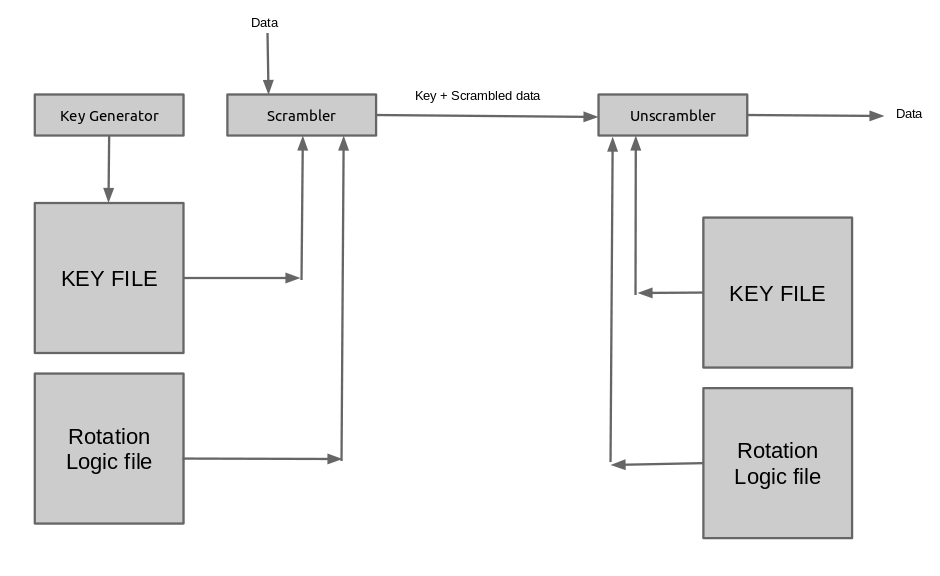
\includegraphics[scale=0.45]{pi.png}
 \caption{Functional Overview of Variable Key Scrambler}
 \label{var_key_overview} %the label was cycle here
\end{figure}

\begin{itemize}
  \item {\bf Key Generator} is the module that generates a key bank file. It is a superset of all the keys that will be used used for scrambling. It is a one time operation. Once key file is generated, it must be securely shared with the intended recipient.
  \item {\bf Scrambler} takes the original data stream and using the rotation string swaps various positions in the data stream as a result the data is jumbled.
  \item {\bf Unscrambler} does the reverse of what scrambler does, it takes the jumbled data and rearranges everything back together.
  \item  {\bf Rotation Logic File} has the definitions and descriptions of how the transformations need
to be implemented.
\end{itemize}

\subsection{Specifications of the Project}

\begin{itemize}
  \item {\bf Key Generator} The module should take the number of actual keys to be generated for the keybank. It should create a set of keys randomly during the time of key generation. Each set of key generated must in turn be random sequences of the defined operations from a Rotation logic file. The output will be the key bank, which should be saved to a file.

  \item {\bf Rotation Logic File} It is mostly pre defined by the algorithm and may not change. They define the “micro-operations” being done on the data. This defines the actual scrambling operation. It is the superset of all known operations that will be used for a scrambling.

  \item {\bf Scrambler/Unscrambler} The scrambler should takes the input from key banks and rotation logic file so as to decide what sequence of keys must be chosen to scramble the current payload data. The unscrambler does the reverse operation on the scrambled data so as to decipher the original data.

\end{itemize}


\subsection{End User}

The target users of this project would be any common users of internet, particularly for
the embedded devices which fall in the category of IoT in which every kind of optimization
that saves computational overhead is important, because we can reduce the computation
time if the payload data is having lesser validity, owing to a simpler encryption.

\section{Implementation}

The proof of concept is being implemented in C. C was chosen for its speed. When it
comes to proving the efficiency of an algorithm, fastest languages is always the best
option.

\subsection{Design Constraints and Dependencies}


\begin{itemize}
  \item {\bf Key Generator} For the key generator program, a limit of 25 was chosen for the horizontal
length in the key file for simplicity. It can be extended to any length. However, longer keys
would mean more computation. Thus the algorithm selects proper key based on how
important the data to be transmitted is. The importance level is selected by the user. Also,
since the length of key depends on importance level of data, the key selected is of proper
size such that the key overhead is avoided.
  
\end{itemize}




\newpage

%\paragraph*{•}
%The main parameters to be discussed are: - 
%\begin{enumerate}
%\item Exhaust Valve Opening Timing - EVO 
%\item  Exhaust Valve Closing Timing – EVC 
%\item  Intake Valve Opening Timing – IVO 
%\item  Intake Valve Closing Timing – IVC 
%\item Peak Valve Lift
%\end{enumerate}

